% Capítulo 2 — Contextualization
% RASCUNHO (Sessão 4). Dados de mercado US 2025–2026, reais e verificados (§6.1).
% Cada afirmação tem fonte verificada (docs/citation_log.md). Rever/editar (o texto é teu).

\chapter{Contextualization}
\label{chap:contextualization}

This chapter sets the context for the work. It outlines the scale of the United States equity market, the
growth of retail investing, the rapid adoption of \gls{AI} in finance and the explainability concerns it
raises, and the information-overload problem that motivates an explainable financial-alert system.

\section{The US Equity Market (NYSE and NASDAQ)}
\label{sec:ctx_market}

The United States equity market is the largest and among the deepest and most liquid in the world. According to
the \gls{SIFMA} Capital Markets Fact Book, US equity markets represented 49.1\% of the US\$126.7~trillion in
global equity market capitalisation at the end of 2024 --- about US\$62.2~trillion, some 5.3 times the size of
the next-largest market, China \autocite{sifma2025factbook}. The two principal trading venues are the
\gls{NYSE} and \gls{NASDAQ}, which together list the large-capitalisation companies that dominate global indices.

This market has also grown substantially over the last decade. As shown in Figure~\ref{fig:us_market_cap}, US
equity market capitalisation rose from US\$25.1~trillion in 2015 to US\$62.2~trillion in 2024
\autocite{sifma2025factbook}, a scale and liquidity that make it the natural focus for a retail-oriented
alerting system.

\begin{figure}[ht]
\centering
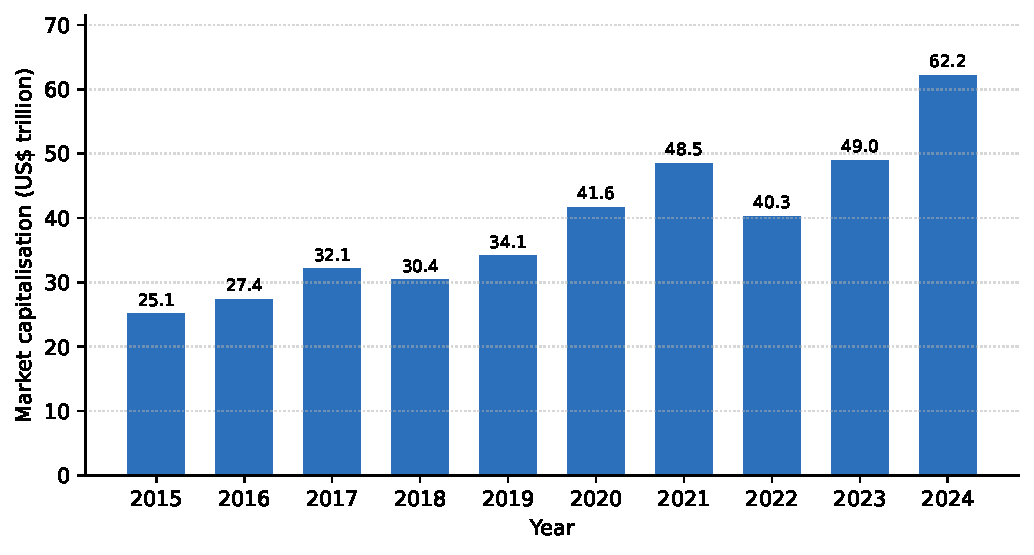
\includegraphics[width=0.9\textwidth]{figures/us_equity_market_cap.pdf}
\caption[US equity market capitalisation, 2015--2024]{US equity market capitalisation, 2015--2024
(US\$~trillion). Figure generated from data reported in the SIFMA 2025 Capital Markets Fact Book
\autocite{sifma2025factbook}.}
\label{fig:us_market_cap}
\end{figure}

\section{The Retail-Investing Landscape}
\label{sec:ctx_retail}

Equity ownership is widespread among US households. In 2025, 62\% of Americans reported owning stock --- whether
individual shares or holdings within mutual funds and retirement accounts --- matching the 2024 figure and
continuing a rebound after more than a decade below that level \autocite{gallup2025stock}. Ownership is, however,
unevenly distributed: it rises to 87\% among households earning US\$100{,}000 or more and falls to 28\% among
those earning under US\$50{,}000 \autocite{gallup2025stock}.

Beyond ownership, individual (``retail'') investors have become a material part of day-to-day trading activity,
helped by commission-free mobile brokerages. Published estimates of the retail share of US equity trading
volume vary widely with methodology and period --- broadly in the range of 20--35\% during 2024--2025.
% TODO (revisão): fixar uma fonte primária única para a quota de retalho no volume (ex.: SIFMA / Cboe / MEMX) e citar com valor exato.
This combination of broad ownership and growing direct participation defines the audience this work serves: the
non-professional investor who must make sense of the market without the tools available to institutions.

\section{Artificial Intelligence in Finance}
\label{sec:ctx_ai_finance}

\Gls{AI} has been adopted rapidly across financial services. A 2026 industry survey by the Cambridge Centre for
Alternative Finance found that 81\% of surveyed financial-services firms were adopting AI at some level, 40\% of
industry respondents reported advanced adoption, and 71\% were already using generative AI
\autocite{ccaf2026aifs}. Typical applications include fraud detection, market analysis and customer service.

This rapid adoption raises a well-documented concern: many high-performing models behave as ``black boxes'',
offering little insight into how a given output was produced. \Gls{XAI} addresses precisely this gap, seeking
methods whose reasoning users can follow and trust \autocite{arrieta2020xai, adadi2018peeking}. For a retail
investor, who must act on --- and bear the consequences of --- a system's output, this transparency is not a
luxury but a requirement. It is the principle that guides the present work.

\section{The Information-Overload Problem}
\label{sec:ctx_problem}

A retail investor faces two simultaneous streams of information: continuous price movements across thousands of
US tickers, and a constant flow of financial news. Distinguishing a meaningful movement from ordinary
volatility, and understanding whether and how a news item is likely to affect an asset, requires time, data and
expertise that most non-professionals do not have.

This is the gap the dissertation addresses. Rather than predicting prices, the proposed system detects abrupt
movements and relevant news, and --- crucially --- explains them: what was detected, the reasoning applied, the
sources, and concrete historical precedents of analogous events and their observed impact. The remainder of the
document develops and evaluates this explainable alerting system.
